\documentclass[]{cpp}
\title{省选基础算法}
\author{雷宇辰}
\renewcommand{\Vec}{\overrightarrow}
\begin{document}
\setcounter{page}{0}
\maketitle
\begin{center}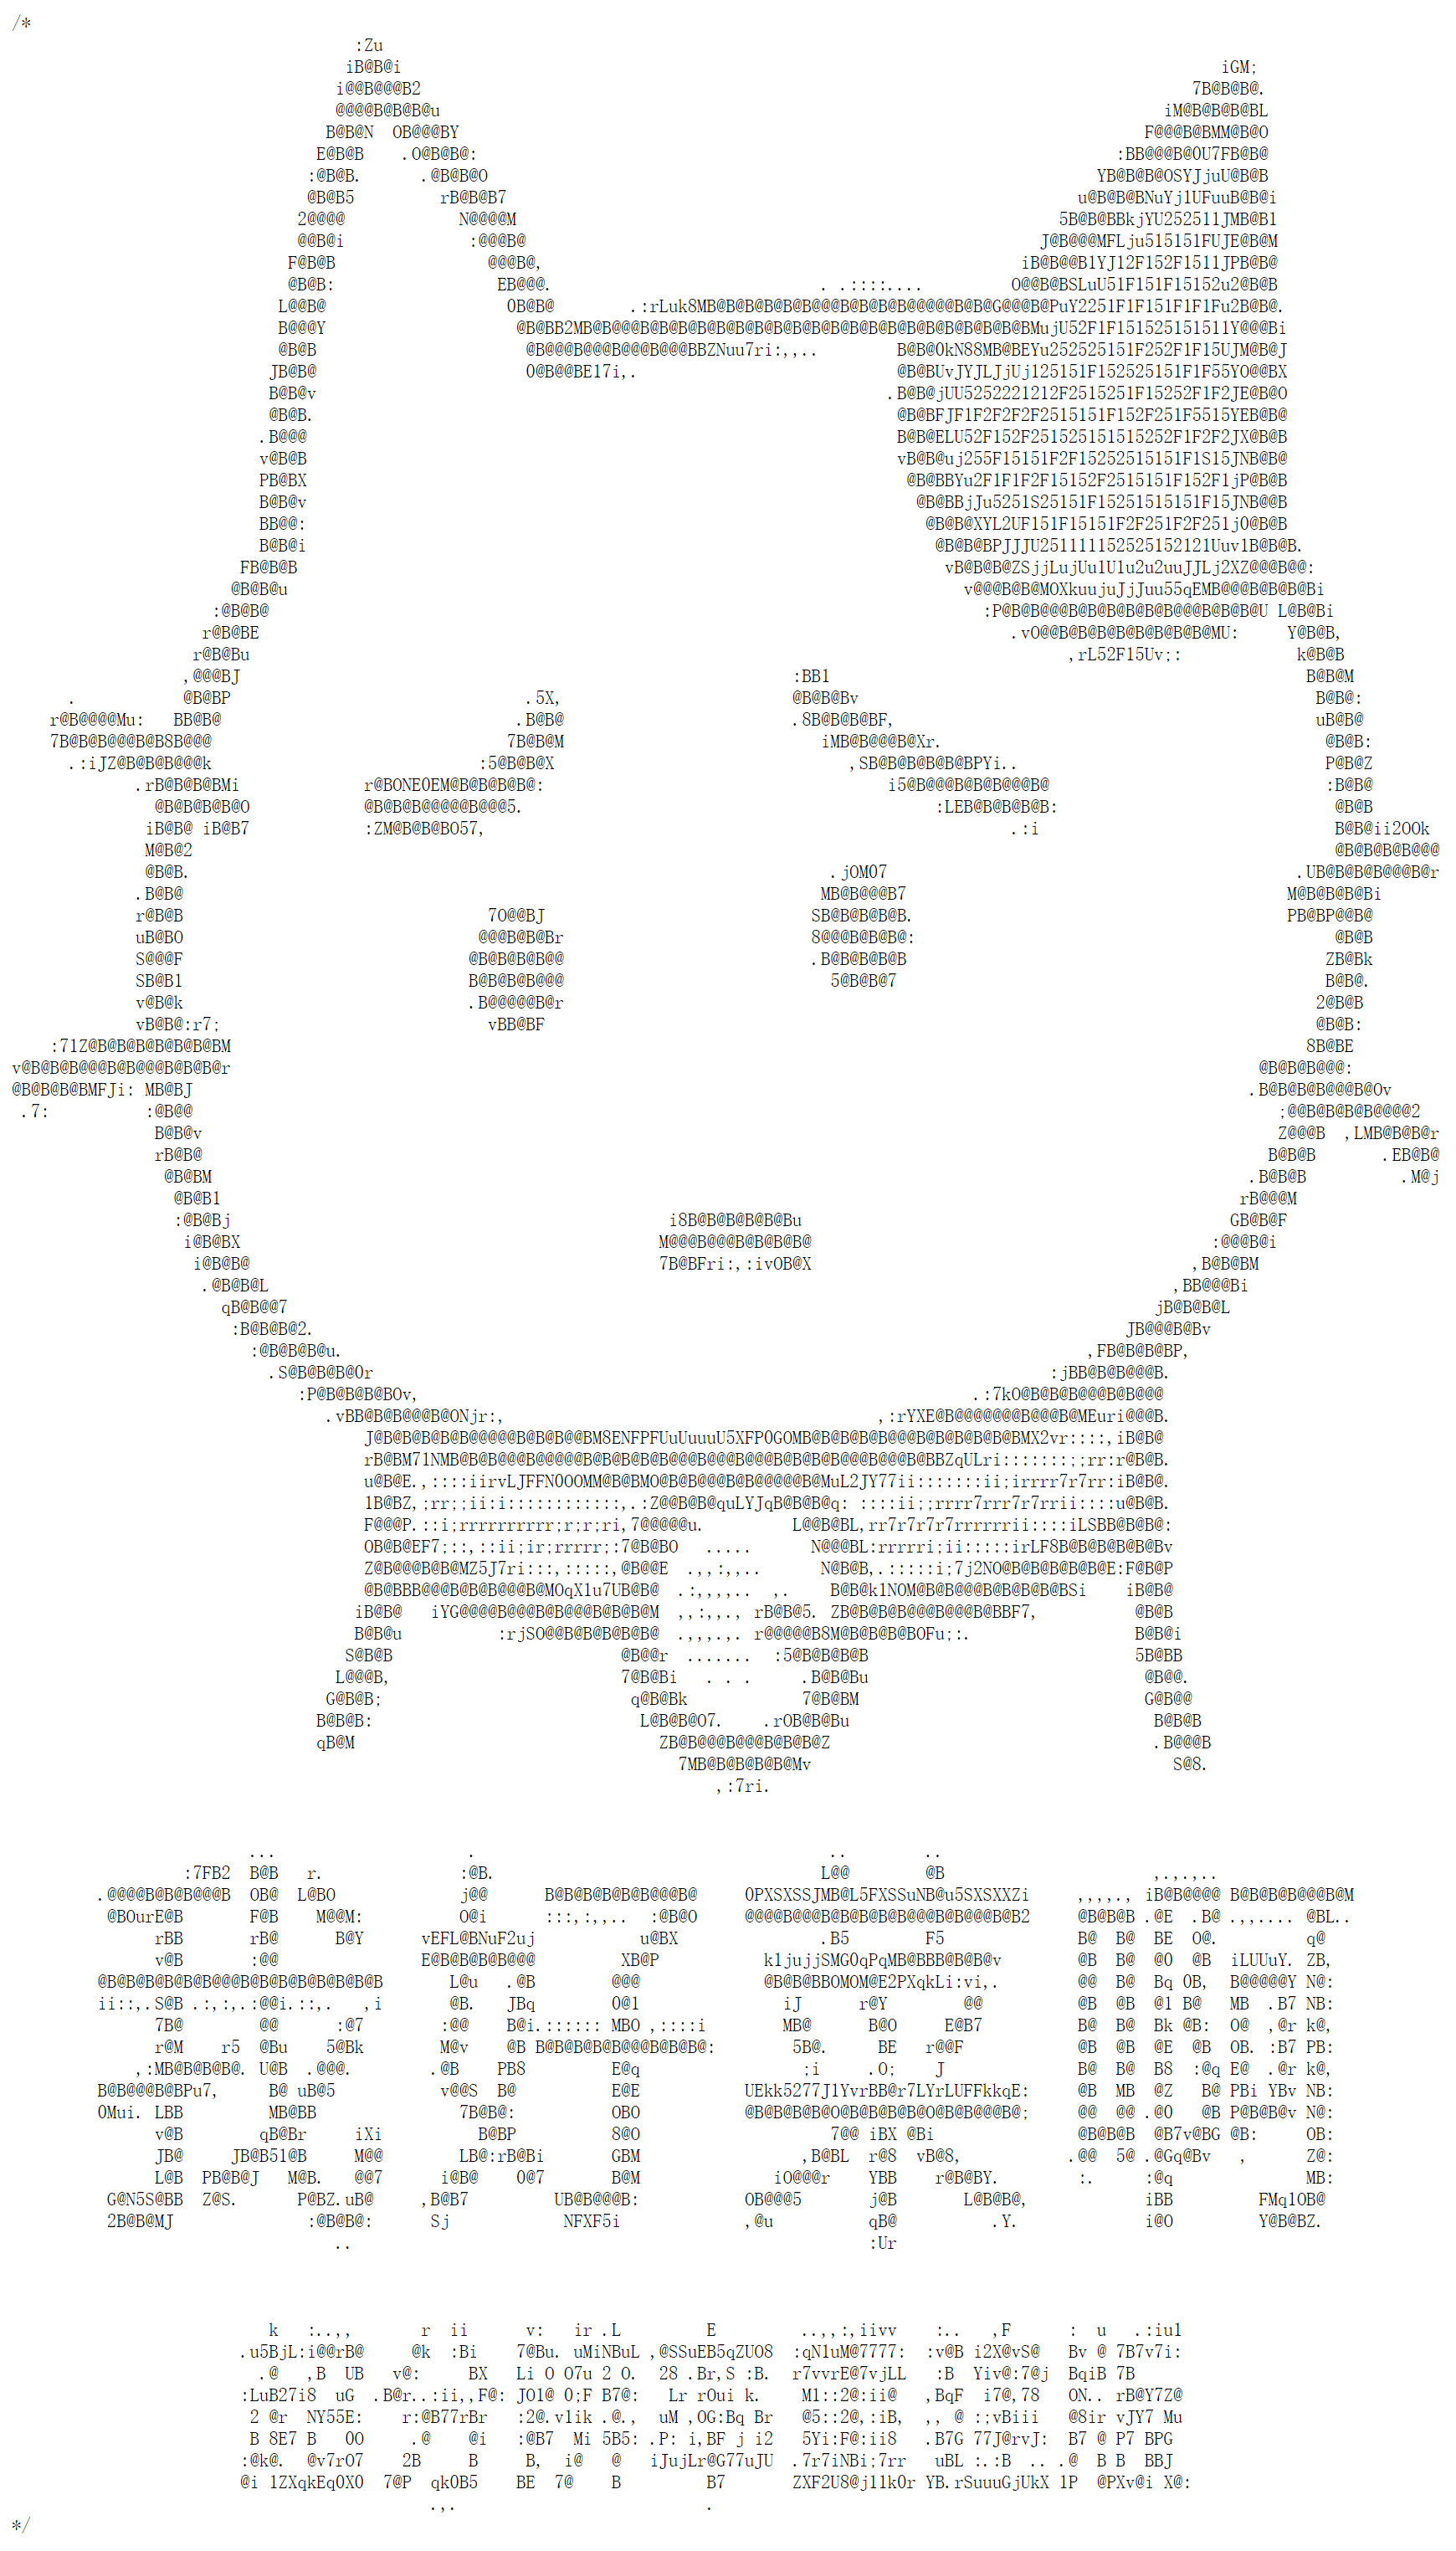
\includegraphics[height=20cm]{assets/banner.png}\end{center}
\newpage
\tableofcontents
\newpage
\setcounter{page}{1}
\section{day1 图论}
\subsection{有向图强连通分量的 Tarjan 算法}
\paragraph{定义}
	在\textbf{有向图$G$}中,如果两个顶点$u,v$间存在一条路径$u$到$v$的路径且也存在一条$v$到$u$的路径,则称这两个顶点$u,v$是\textbf{强连通的(strongly connected)}。如果有向图$G$的每两个顶点都强连通,称$G$是一个\textbf{强连通图}。有向非强连通图的 极大强连通子图,称为\textbf{强连通分量(strongly connected components)}。若将有向图中的强连通分量都缩为一个点,则原图会形成一个 DAG(有向无环图)。
\subparagraph{极大强连通子图}
	$G$是一个极大强连通子图当且仅当$G$是一个强连通子图且不存在另一个强连通子图$G'$使得$G$是$G'$的真子集。
\paragraph{Tarjan 算法}
	定义$dfn(u)$为结点$u$搜索的次序编号,给出函数$low(u)$使得\\
	$low(u) = min$
	\\$\{$\\
	\verb|    |$dfn(u),$\\
	\verb|    |$low(v),$  \quad $(u,v)$为树枝边,$u$为$v$的父结点\\
	\verb|    |$dfn(v)\;$ \quad $(u,v)$为后向边或指向栈中结点的横叉边
	\\$\}$\\
	当结点$u$的搜索过程结束后,若$dfn(u)=low(u)$,则以$u$为根的搜索子树上所有还在栈中的结点是一个强连通分量。
\subparagraph{代码}$\\$
\codeinput[tarjan - SCC]{assets/day1/tarjan-scc.cpp}
\paragraph{练习题}
\subparagraph{\href{http://poj.org/problem?id=2186}{POJ2186}/\href{http://www.lydsy.com/JudgeOnline/problem.php?id=1051}{BZOJ1051} - Popular Cows} 双倍的快乐
\codeinput[Popular Cows]{assets/day1/poj2186.cpp}
\subparagraph{\href{http://poj.org/problem?id=3180}{POJ3180} - The Cow Prom} The $N (2 <= N <= 10,000)$ cows are so excited.
\codeinput[The Cow Prom]{assets/day1/poj3180.cpp}
\subparagraph{\href{http://poj.org/problem?id=3180}{POJ1236} - Network of Schools} 强连通分量缩点求出度为0的和入度为0的分量个数
\codeinput[Network of Schools]{assets/day1/poj1236.cpp}
\subsection{图的割点、桥与双连通分量}
\paragraph{定义}
\subparagraph{点连通度与边连通度}
	在一个\textbf{无向连通图}中,如果有一个顶点集合$V$,删除顶点集合$V$,以及与$V$中顶点相连(至少有一端在$V$中)的所有边后,原图\textbf{不连通},就称这个点集$V$为\textbf{割点集合}。\\
	一个图的\textbf{点连通度}的定义为:最小割点集合中的顶点数。\\
	类似的,如果有一个边集合,删除这个边集合以后,原图不连通,就称这个点集为\textbf{割边集合}。
\subparagraph{双连通图、割点与桥}
	如果一个无向连通图的\textbf{点连通度大于$1$},则称该图是\textbf{点双连通的(point biconnected)},简称双连通或重连通。一个图有\textbf{割点},当且仅当这个图的点连通度为$1$,则割点集合的唯一元素被称为\textbf{割点(cut point)},又叫关节点(articulation point)。一个图可能有多个割点。\\
	如果一个无向连通图的\textbf{边连通度大于$1$},则称该图是\textbf{边双连通的(edge biconnected)},简称双连通或重连通。一个图有\textbf{桥},当且仅当这个图的边连通度为$1$,则割边集合的唯一元素被称为\textbf{桥(bridge)},又叫关节边(articulation edge)。一个图可能有多个桥。\\
	可以看出,点双连通与边双连通都可以简称为双连通,它们之间是有着某种联系的,下文中提到的双连通,均既可指点双连通,又可指边双连通。(但这并不意味着它们等价)\\
	双连通分量(分支):在图$G$的所有子图$G'$中,如果$G'$是双连通的,则称$G'$为双连通子图。如果一个双连通子图$G'$它不是任何一个双连通子图的真子集,则$G'$为极大双连通子图。双连通分量(biconnected component),或重连通分量,就是图的极大双连通子图。特殊的,点双连通分量又叫做块。
\paragraph{Tarjan 算法}
	给出函数$low(u)$使得\\
	$low(u) = min$
	\\$\{$\\
	\verb|    |$dfn(u),$\\
	\verb|    |$low(v),$  \quad $(u,v)$为树枝边(父子边)\\
	\verb|    |$dfn(v)\;$ \quad $(u,v)$为后向边(返祖边) 等价于$dfn(v)<dfn(u)$且$v$不为$u$的父亲结点
	\\$\}$\\
\subparagraph{代码}$\\$
\codeinput[tarjan - BCC]{assets/day1/tarjan-bcc.cpp}
\paragraph{练习题}
\subparagraph{\href{http://poj.org/problem?id=3177}{POJ3177} - Redundant Paths}
将一张有桥图通过加边变成边双连通图,至少要加$\frac{leaf+1}{2}$条边。
\codeinput[Redundant Paths]{assets/day1/poj3177.cpp}
\subparagraph{\href{http://poj.org/problem?id=1523}{POJ1523} - SPF}
求割点与删除这个点之后有多少个连通分量
\codeinput[Redundant Paths]{assets/day1/poj1523.cpp}
\subparagraph{\href{http://poj.org/problem?id=2942}{POJ2942} - Knights of the Round Table}
这题过于复杂,我来先给个\href{http://blog.csdn.net/lyy289065406/article/details/6756821}{别人的题解}。然后是我自己的实现(仿佛还是没看懂。
\\ //实现被狗吃了
%\codeinput[Knights of the Round Table]{assets/day1/poj2942.cpp}
\subsection{2-SAT}
\paragraph{定义}
	给定一个布尔方程,判断是否存在一组布尔变量的取值方案,使得整个方程值为真的问题,被称为布尔方程的可满足性问题(SAT)。SAT问题是NP完全的,但对于一些特殊形式的SAT问题我们可以有效求解。\\
	我们将下面这种布尔方程称为合取范式:
	$$(a\lor b\lor c\lor\cdots)\land(d\lor e\lor f\lor\cdots)\land\cdots$$
	其中$a,b,c,\cdots$称为文字,它是一个布尔变量或其否定。像$(a\lor b\lor c\lor\cdots)$这样用$\lor$连接的部分称为子句。如果合取范式的每个子句中的文字个数都不超过两个,那么对应的SAT问题又称为\textbf{2-SAT}问题。
\paragraph{解法}
	对于给定的\textbf{2-SAT}问题,首先利用$\Rightarrow$将每个子句$(a\lor b)$改写成等价形式$(\neg a\Rightarrow b\land a\Rightarrow\neg b)$.这样原布尔公式就变成了把$a\Rightarrow b$形式的布尔公式用$\land$连接起来的形式。\\
	对每个布尔变量$x$构造两个顶点分别代表$x$与$\neg x$。以$\Rightarrow$关系为边建立有向图。若在此图中$a$点能到达$b$点,就表示$a$为真时$b$也一定为真。因此该图中同一个强连通分量中所含的所有变量的布尔值均相同。\\
	若存在某个变量$x$,代表$x$与$\neg x$的两个顶点在同一个强连通分量中,则原布尔表达式的值无法为真。\\
	反之若不存在这样的变量,那么我们先将原图中所有的强连通分量缩为一个点,构出一个新图,新图显然是一个拓扑图,我们求出它的一个拓扑序。那么对于每个变量$x$,\textbf{$$x\text{所在的强连通分量(新图中的点)的拓扑序在}\neg x\text{所在的强连通分量之后}\Leftrightarrow x\text{为真}$$}就是一组合适布尔变量赋值。注意到 Tarjan 算法所求的强连通分量就是按拓扑序的逆序得出的,因此不需要真的缩点建新图求拓扑序,直接利用强连通分量的编号来当做顺序即可。
\paragraph{练习题}
\subparagraph{\href{http://poj.org/problem?id=3648}{POJ3648} - Wedding}
Additionally, there are several pairs of people conducting adulterous relationships (both different-sex and same-sex relationships are possible)
\codeinput[adulterous relationships]{assets/day1/poj3648.cpp}
\subparagraph{\href{http://poj.org/problem?id=3678}{POJ3678} - Katu Puzzle} 我什么时候做过这个题?
\codeinput[Katu Puzzle]{assets/day1/poj3678.cpp}
\subparagraph{\href{http://poj.org/problem?id=2749}{POJ2749} - Building roads} 杀光奶牛问题就会得到解决
\codeinput[Building roads]{assets/day1/poj2749.cpp}
\subsection{欧拉回路}
\paragraph{定义}
	设$G=(V,E)$是一个图。
\subparagraph{欧拉回路} 图$G$中经过\textbf{每条边一次}并且\textbf{仅一次}的回路称作欧拉回路。
\subparagraph{欧拉路径} 图$G$中经过\textbf{每条边一次}并且\textbf{仅一次}的路径称作欧拉路径。
\subparagraph{欧拉图}   存在\textbf{欧拉回路}的图称为欧拉图。
\subparagraph{半欧拉图} 存在欧拉路径但不存在欧拉回路的图称为半欧拉图。
\paragraph{性质与定理}
	以下不加证明的给出一些定理\quad\sout{(因为我懒得抄讲义了}
\subparagraph{定理 1} 无向图$G$为欧拉图,当且仅当$G$为连通图且所有顶点的度为偶数。
\subparagraph{推论 1} 无向图$G$为半欧拉图,当且仅当$G$为连通图且除了两个顶点的度为奇数之外,其它所有顶点的度为偶数。
\subparagraph{定理 2} 有向图$G$为欧拉图,当且仅当$G$的基图\footnote{忽略有向图所有边的方向,得到的无向图称为该有向图的基图。}连通,且所有顶点的入度等于出度。
\subparagraph{推论 2} 有向图$G$为半欧拉图,当且仅当$G$的基图连通,且存在顶点$u$的入度比出度大1、$v$的入度比出度小1,其它所有顶点的入度等于出度。
\paragraph{解法}
	由此可以得到以下求欧拉图$G$的欧拉回路的算法:
	\begin{enumerate}
		\item 在图$G$中任意找一个回路$C$。
		\item 将图$G$中属于回路$C$的边删除
		\item 在残留图的各极大连通子图中分别寻找欧拉回路。
		\item 将各极大连通子图的欧拉回路合并到$C$中得到图$G$的欧拉回路。
	\end{enumerate}
	该算法的伪代码如下:
	\begin{verbatim}
	void dfs(u)
	{
	    for (edge e : edges[u])
	        if (!flag[e])
	        {
	            flag[e] = true;
	            flag[rev(e)] = true; //如果图 G 是有向图则删去本行
	            dfs(e.to);
	            S.push(v);
	        }
	}
	\end{verbatim}
	最后依次取出栈$S$每一条边而得到图$G$的欧拉回路(也就是边出栈序的逆序)。由于该算法执行过程中每条边最多访问两次,因此该算法的时间复杂度为$O(|E|)$。
\paragraph{练习题}
\subparagraph{\href{http://uoj.ac/problem/117}{UOJ117} - 欧拉回路}
混合两个子任务使代码风格变得鬼畜起来。
\codeinput[Building roads]{assets/day1/uoj117.cpp}
\section{day2 字符串(一)}
\subsection{KMP}
\paragraph{算法介绍} 用来在线性时间内匹配字符串
\paragraph{算法流程}
	我觉得鏼鏼鏼在WC上讲的比较清楚,于是我开始抄讲义。\\
	\textbf{字符串:} $s[1\ldots n]$, $|s| = n$。\\
	\textbf{子串:} $s[i\ldots j] = s[i]s[i + 1]\cdots[j]$。\\
	\textbf{前缀:} $pre(s,x) = s[1\ldots x]$, 后缀:$suf(s,x) = s[n − x + 1\ldots n]$\\
	若 $0 \leq r \le |s|, pre(s,r) = suf(s,r)$, 就称 $pre(s,r)$ 是 $s$ 的 \textbf{border}。\\
	KMP算法的第一步主要做这么一件事:在$O(n)$时间求出数组$next[1\ldots n]$, 其中$next[i]$表示前缀$s[1\ldots i]$的最大 border 长度。
	于是可以知道$s$的所有 border 长度为${next[n],next[next[n]],\cdots}$,我想这是显然的,于是不加证明的在这里给出。\\
	第二步就是匹配,如果失配了就把模式串的当前位置指针$i$跳到$next[i]$处然后继续匹配,然后就好了。
\paragraph{算法实现}$\\$
\codeinput[genNext]{assets/day2/kmp-genNext.cpp}
\codeinput[Find]{assets/day2/kmp-Find.cpp}
\paragraph{练习题}
\subparagraph{\href{http://poj.org/problem?id=3461}{POJ3461} - Oulipo} 求出所有匹配位置
\codeinput[Oulipo]{assets/day2/poj3461.cpp}
\subparagraph{\href{http://poj.org/problem?id=2406}{POJ2406} - Power Strings} $next$数组的奇妙性质
\codeinput[Power Strings]{assets/day2/poj2406.cpp}
\subparagraph{\href{http://codeforces.com/problemset/problem/526/D}{CF526D} - Om Nom and Necklace} 啥?
\codeinput[Om Nom and Necklace]{assets/day2/CF526D.cpp}
讲道理我KMP真的学的不是很明白,望各位dalao给予指导。
\subsection{Trie}
\paragraph{简介}
	字典树,也称 Trie、字母树,指的是某个字符串集合对应的形如下图的有根树。树的每条边上对应有恰好一个字符,每个顶点代表从根到该节点的路径所对应的字符串(将所有经过的边上的字符按顺序连接起来)。
\paragraph{实现} 水
\codeinput[Trie - impl]{assets/day2/trieImpl.cpp}
\paragraph{练习题}
\subparagraph{\href{http://poj.org/problem?id=3630}{POJ3630} - Phone List}
若插入过程中,有某个经过的节点带有串结尾标记,则之前插入的某个串是当前串的前缀。
\codeinput[Oulipo]{assets/day2/poj3630.cpp}
\subparagraph{\href{http://poj.org/problem?id=2945}{POJ2945} - Find the Clones} 
$n$个基因片段,每个长度为$m$,输出$n$行表示重复出现$i$次$(1 \leq i \leq n)$的基因片段的个数
\codeinput[Find the Clones]{assets/day2/poj2945.cpp}
\subsection{Aho–Corasick Automaton}
\paragraph{简介}
	多模式串字符串匹配,Trie上的KMP,其中$next$数组变成了$fail$指针,功能相同。
\paragraph{实现}
	Trie的实现上文已经出现,所以此处不再重复。
\codeinput[buildFail]{assets/day2/AC-buildFail.cpp}
\paragraph{练习题}
\subparagraph{\href{http://acm.hdu.edu.cn/showproblem.php?pid=2222}{HDU2222} - Keywords Search}
AC 自动机模板题,注意统计答案时,每个节点只能统计一次不要重复统计。
\codeinput[Keywords Search]{assets/day2/hdu2222.cpp}
\subsection{Manacher}
求出字符串每一位的回文半径,算法流程奥妙重重,不易让常人理解,然后我就抄了份板子改了改,然后就比讲义上的标程快了$20\%$。
\paragraph{练习题}
\subparagraph{\href{http://poj.org/problem?id=3974}{POJ3974} - Palindrome}
Manacher 模板题
\codeinput[Palindrome]{assets/day2/poj3974.cpp}
\section{day3 简单数学}
说是简单数学其实我后半部分也没看懂\\
\subsection{整除及剩余}
\paragraph{整除定义}
	设$a,b$是两个整数,且$b\neq0$.如果存在整数$c$,使得$a=bc$,则称$a$被$b$整除,或$b$整除$a$,记作$b|a$。此时,又称$a$是$b$的倍数,$b$是$a$的因子。
\paragraph{整除的基本性质}
	\begin{enumerate}
		\item $a|b \land a|c \Rightarrow a|(b+c)$
		\item $a|b \Rightarrow \forall c\in\mathbb{Z},\ a|bc$
		\item $a|b \land b|c \Rightarrow a|c$
	\end{enumerate}
\paragraph{同余基本定义和定理}
\subparagraph{定义1:带余除法}
	$$\forall a\in\mathbb{Z},b\in\mathbb{Z^{*}}\to\exists q,r\in\mathbb{Z},a=qb+r,r\in [0,|b|)$$
\subparagraph{定义2:同余}
	$$a\!\!\!\!\mod m = b\!\!\!\!\mod m \iff a\equiv b\!\!\!\!\pmod{m}$$
\subparagraph{定义3:剩余类}
	$$\mathbf{A_i}=\{x|x\in\mathbb{Z}\land x\!\!\!\!\mod{m} = i\}\to\forall a,b\in\mathbf{A_i},a\equiv b\!\!\!\!\pmod{m}$$
\subparagraph{定义4:完系}
	$$\{a_1\!\!\!\!\mod m,a_2\!\!\!\!\mod m,\ldots,a_n\!\!\!\!\mod m\}=\{0,1,2,\ldots,m-1\}$$
\subparagraph{定理1}
	$$a\equiv b\!\!\!\!\pmod{m}\iff\exists k\in\mathbb{Z},a=b+km\iff m|(a-b)$$
\subparagraph{定理2} 同余关系是等价关系
	\begin{enumerate}
		\item $a\equiv a\pmod{m}$
		\item $a\equiv b\pmod{m}\Rightarrow b\equiv a\pmod{m}$
		\item $a\equiv b\pmod{m} \;\land\; b\equiv c\pmod{m}\Rightarrow a\equiv c\pmod{m}$
	\end{enumerate}
\subparagraph{定理3} 同余的三则运算\\
	$a,b,c\in\mathbb{R},m\in\mathbb{N^*}, a\equiv b\pmod{m} \Rightarrow$
	\begin{enumerate}
		\item $a+c\equiv b+c\pmod{m}$
		\item $a-c\equiv b-c\pmod{m}$
		\item $ac\equiv bc\pmod{m}$
	\end{enumerate}
\subparagraph{定理4} 同余式的三则运算\\
	$a,b,c\in\mathbb{R},m\in\mathbb{N^*}, a\equiv b\pmod{m} \land c\equiv d\pmod{m} \Rightarrow$
	\begin{enumerate}
		\item $ax+cy\equiv bx+dy\pmod{m}\qquad x,y\in\mathbb{Z}$
		\item $ac\equiv bd\pmod{m}$
		\item $a^n\equiv b^n\pmod{m}\qquad n\in\mathbb{N^*}$
		\item $f(a)\equiv f(b)\pmod{m}\qquad f(x)$为任一整系数多项式
	\end{enumerate}
\subparagraph{定理5}
	\begin{enumerate}
		\item $a\equiv b\pmod{m}\land d|m \Rightarrow a\equiv b\pmod{d}$
		\item $a\equiv b\pmod{m}\Rightarrow gcd(a,m)=gcd(b,m)$
		\item $\forall i \in [1,n]\ ,\;a\equiv b\pmod{m_i} \iff a\equiv b\pmod{lcm(m_1,m_2,\ldots,m_n)}$
	\end{enumerate}
\subsection{素数}
\paragraph{定义}
	素数(质数)是大于$1$的正整数,并且除了$1$和它本身不能被其他正整数整除。大于$1$的非素数的正整数称为合数。
\paragraph{分布}
	素数有无穷多个.如果使用$\pi(x)$表示小于一个正实数$x$的素数有多少个,那么有$$\lim\limits_{x\rightarrow{\infty}}\frac{\pi(x)}{x}=\ln{x}$$
\paragraph{算术基本定理/惟一分解定理}
	$$n=\prod\limits_{i=1}^\infty p_i^{a_i} \qquad p_i\in\mathbb{P},\;a_i\in\mathbb{N}$$
\paragraph{判定}
	$$n\in\mathbb{P}\iff\forall i\in[2,\sqrt{n}],\;i\nmid n$$
\paragraph{Eratosthenes 筛法} $ $
\codeinput[Eratosthenes Sieve]{assets/day3/Eratosthenes.cpp}
\paragraph{欧拉函数} 欧拉函数$\varphi(n)$指不超过$n$且与$n$互素的正整数的个数,其中$n$是一个正整数。
\subparagraph{欧拉函数的性质} $n=\prod\limits_{i=1}^m p_i^{a_i}\to\varphi(n)=\prod\limits_{i=1}^m\varphi(p_i^{a_i})$
\subparagraph{定理1} $p\in\mathbb{P}\iff\varphi(p)=p-1$
\subparagraph{定理2} $p\in\mathbb{P},\;a\in\mathbb{N_+}\Rightarrow\varphi(p^a)=p^{a}-p^{a-1}$
\subparagraph{定理3} $m,n\in\mathbb{N_+}\land gcd(m,n)=1\Rightarrow\varphi(mn)=\varphi(m)\varphi(n)$
\subparagraph{定理4} $n=\prod\limits_{i=1}^m p_i^{a_i}\to\varphi(n)=n\prod\limits_{i=1}^{m}(1-\frac{1}{p_i})$
\subparagraph{推论} $n\equiv1\pmod2\to\varphi(2n)=\varphi(n)$
\subparagraph{定理5} $n\in(2,+\infty)\bigcap\mathbb{Z}\Rightarrow\varphi(n)\equiv0\pmod2$
\subparagraph{定理6} $n\in\mathbb{N_+}\Rightarrow\sum\limits_{d|n}\varphi(n)=n$
\subparagraph{欧拉定理} $gcd(a,m)=1,a\in\mathbb{N_+},m\in[2,+\infty)\bigcap\mathbb{Z}\Rightarrow a^{\varphi(m)}\equiv1\pmod{m}$
\subparagraph{费马小定理} $m\in\mathbb{P}\Rightarrow a^{m-1}\equiv1\pmod{m}$
\paragraph{练习题}
\subparagraph{\href{http://poj.org/problem?id=2689}{POJ2689} - Prime Distance} 暴力筛掉合数
\codeinput[Prime Distance]{assets/day3/poj2689.cpp}
\subparagraph{\href{http://poj.org/problem?id=3421}{POJ3421} - X-factor Chains} 质因子的排列组合
\codeinput[X-factor Chains]{assets/day3/poj3421.cpp}
\subparagraph{\href{http://poj.org/problem?id=3090}{POJ3090} - Visible Lattice Points} 欧拉函数
\codeinput[Visible Lattice Points]{assets/day3/poj3090.cpp}
\subsection{欧几里得算法}
\paragraph{最大公约数与最小公倍数}
\subparagraph{定义1} 设$a$和$b$是两个整数,如果$d|a$ 且$d|b$,则称$d$是$a$与$b$的公因子
\subparagraph{定义2} 设$a$和$b$是两个不全为$0$的整数,称$a$与$b$的公因子中最大的为$a$与$b$的最大公因子,或最大公约数,记作$gcd(a,b)$
\subparagraph{定义3} 设$a$和$b$是两个非零整数,称$a$与$b$最小的正公倍数为$a$与$b$的最小公倍数,记作$lcm(a,b)$
\paragraph{最大公约数与最小公倍数的性质}
	\begin{enumerate}
		\item $a|m \land b|m \Rightarrow lcm(a,b)|m$
		\item $d|a \land d|b \Rightarrow d|gcd(a,b)$
		\item $lcm(a,b)=\frac{ab}{gcd(a,b)}$
		\item $m,a,b\in\mathbb{N_+}\to lcm(ma,mb)=m\times lcm(a,b)\ ,\;\ gcd(ma,mb)=m \times gcd(a,b)$
	\end{enumerate}
\paragraph{计算方法}
\subparagraph{素因子分解法}
	令 $$a=\prod\limits_{i=1}^{m}p_{i}^{r_i}\;,\quad\;b=\prod\limits_{i=1}^{m}p_{i}^{s_i}$$
	于是 $$gcd(a,b)=\prod\limits_{i=1}^{m}p_{i}^{min(r_i,s_i)}\;,\quad\;lcm(a,b)=\prod\limits_{i=1}^{m}p_{i}^{max(r_i,s_i)}$$
\subparagraph{欧几里得算法1} $$gcd(a,b)=gcd(b,a\!\!\!\!\mod b)$$
\subparagraph{欧几里得算法2} $$gcd(a,b)=gcd(a,a-b)$$
\paragraph{拓展欧几里得算法} 不理解就记下来
\codeinput[exgcd]{assets/day3/exgcd.cpp}
\subsection{线性同余方程}
\paragraph{二元一次不定方程}
\subparagraph{定义1} $a,b,c\in\mathbb{Z},a\ne0,b\ne0$,那形如$ax+by=c$的方程称为二元一次不定方程。
\subparagraph{定理1} 设$a,b\in\mathbb{Z}$且$d=gcd(a,b)$,如果$d|c$,那么方程存在无穷多个整数解,否则方程不存在整数解。
\subparagraph{定理2} 如果不定方程有解且特解为$x=x_0,y=y_0$那么方程的解可以表示为$$x=x_0+\frac{b}{d}t,y=y_0-\frac{a}{d}t,\mbox{其中}t\in\mathbb{Z}$$
\paragraph{同余方程与不定方程} 在$a>0$且$b>0$的条件下,求二元一次方程$ax+by=c$的整数解等价于求一元线性同余方程$ax\equiv c\bmod{b}$的整数解
\paragraph{求一元线性同余方程}
	要求$ax\equiv c\bmod{b}$,即为求$ax+my=b$的解。记$d=gcd(a,m)$,先使用拓展欧几里得求$ax+my=b$,如果$d\nmid b$则无解,否则$\mod m$意义下的解有$d$个,可以通过对其中某个解不断地加$\frac{m}{d}$得到。(这$d$个解的形式为$x_0+\frac{m}{d}t,\;t\in\mathbb{Z}$,其中$x_0$是已知的一个解)
\paragraph{中国剩余定理}
	若$m_1,m_2,m_3,\ldots,m_r$是两两互素的正整数,则同余方程组
	\begin{equation}
	\left\{\begin{aligned}
		& x\equiv a_1\pmod{m_1}\\
		& x\equiv a_2\pmod{m_2}\\
		& x\equiv a_3\pmod{m_3}\\
		& \cdots\\
		& x\equiv a_r\pmod{m_r}\\
	\end{aligned}\right.
	\end{equation}
	有$\mod M=\prod\limits_1^r m$的唯一解,即为中国剩余定理。\\
	若$n=pq$且$gcd(p,q)=1$,那么$x\mod p,x\mod q$的值确定后,$x\mod n$的值也会随之确定。
\subparagraph{算法说明}
	$$M_i=\prod\limits_{j\ne i}m_j\to gcd(M_i,m_i)=1\Rightarrow \exists p_i,q_i,\,M_ip_i+m_iq_i=1$$
	$$(e_i=M_i p_i)\equiv int(j==i)\pmod{m_i} \to \sum\limits_1^r e_i a_i\mod{\sum\limits_1^r m_i}\mbox{是方程的最小非负整数解}$$
\paragraph{练习题}
\subparagraph{\href{http://poj.org/problem?id=1061}{POJ1061} - 蛤蛤的约会} +1s
\codeinput[蛤蛤的约会]{assets/day3/poj1061.cpp}
\subparagraph{\href{http://poj.org/problem?id=2142}{POJ2142} - The Balance} 求$ax+by=c$的一组解,使得$|x|+|y|$尽量小,在前者尽量小时$|ax|+|by|$尽量小
\codeinput[The Balance]{assets/day3/poj2142.cpp}
\subsection{逆元}
\paragraph{解一元线性同余方程}
	$$gcd(a,m)=1\Rightarrow\exists x,ax\equiv1\pmod{m}$$
	$$ax\equiv1\pmod{m}\iff\exists k\in\mathbb{Z},\,ax-km=1$$
\codeinput[\ ]{assets/day3/inv.cpp}
\paragraph{费马小定理}
	$$\forall p\in\mathbb{P}\to x^p\equiv x\pmod{p}$$被称为费马小定理,若$p\nmid x$,有
	$$x^{p-1}\equiv 1\pmod{p}$$于是有
	$$\forall p\in\mathbb{P},x\in\mathbb{Z}\to x^{-1}\equiv x^{p-2}\pmod{p}$$
	使用快速幂即可计算。
\subsection{离散对数问题}
	解这鬼东西:$$A^x\equiv B\pmod{C}$$ 这玩意有个性质,$A^x\mod C$有周期性,最大周期不超过$C$,我想这是显然的(除非你没上过小学)。
\paragraph{$C\in\mathbb{P}$}
	普通的BSGS
\subparagraph{\href{http://poj.org/problem?id=2417}{POJ2417} - Discrete Logging} 模板题
\codeinput[Primitive Roots]{assets/day3/poj2417.cpp}
\paragraph{$C\in\mathbb{N_+}$}
	待续
\subsection{原根}
\paragraph{阶}
	$$n>1,a\in\mathbb{Z},gcd(a,n)=1\to\exists r\in[1,n],a^r\equiv1\pmod{n}$$ $r$的最小整数值称为$a$模$n$的阶,记为$Ord_n(a)$
\paragraph{阶的性质}
	$$gcd(a,n)=1,r=Ord_n(a),\forall N\in\{x|a^N\equiv1\pmod{n}\}\Rightarrow r|N$$
	$$gcd(a,n)=1\Rightarrow Ord_n(a)|\varphi(n)$$
	$$\mbox{特别的,}p\in\mathbb{P},gcd(a,p)=1\Rightarrow Ord_p(a)|p-1\mbox{,显然}\varphi(p)=p-1$$
\paragraph{原根} $n\in\mathbb{N_+},a\in\mathbb{Z},Ord_n(a)=\varphi(n)$,则称$a$为模$n$的一个原根,由阶的定义可知原根和$n$必然互质。
\paragraph{求质数$p$的原根算法} 暴力从小到大枚举$g\in\mathbb{N_+}$,$\forall a\in\{x\;|\;x|p-1,x\in\mathbb{P}\},g^{\frac{p-1}{a}}\not\equiv1\pmod{p}$
\codeinput[Primitive Root]{assets/day3/proot.cpp}
\paragraph{练习题}
\subparagraph{\href{http://poj.org/problem?id=1284}{POJ1284} - Primitive Roots} 如果$n\in\mathbb{N_+}$有一个原根,那么$n$一共有$\varphi(\varphi(n))$个不同余的原根
\codeinput[Primitive Roots]{assets/day3/poj1284.cpp}
\section{day4 数据结构}
\subsection{树状数组} 在$\lg{n}$的时间内更新或查询$\sum\limits_{i=1}^n a_i$
\paragraph{lowbit} \verb|lowbit(x) = x & -x|
\paragraph{两个操作} $\lg{n}$更新或查询
\codeinput[Fenwick tree]{assets/day4/FenwickTree.cpp}
\paragraph{练习题}
\subparagraph{\href{http://poj.org/problem?id=2352}{POJ2352} - Stars} 。。。
\codeinput[Stars]{assets/day4/poj2352.cpp}
\subparagraph{\href{http://poj.org/problem?id=2299}{POJ2299} - Ultra-QuickSort} 求逆序对数量,不过配图是啥玩意?马桶橛子?
\codeinput[Ultra-QuickSort]{assets/day4/poj2299.cpp}
\begin{center}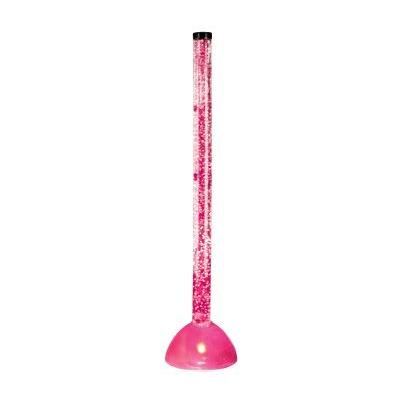
\includegraphics[height=10cm]{assets/day4/poj2299.jpg}\end{center}
\subparagraph{\href{http://poj.org/problem?id=1990}{POJ1990} - MooFest} 杀光奶牛问题就会得到解决
\codeinput[MooFest]{assets/day4/poj1990.cpp}
\subsection{Sparse Table} 处理区间最值,即 RMQ(Range Minimum Query)问题。
\paragraph{预处理} 计算一个数组$f$,使$f[i][j]=min[i,i+2^j)$,然后你就可以开始倍增了。
	\begin{eqnarray}
	f[i][j]=\left\{\begin{array}{lr}
		a[i] & j=0 \\
		min(f[i][j-1],f[i+2^{j-1}][j-1]) & j>0
		\end{array}\right.
	\end{eqnarray}
\paragraph{询问}
	考虑一个询问区间$[x,y)$的最小值的询问操作。\\
	我们可以求出满足$2^i\le y-x < 2^{i+1}$的$i$,即$\lfloor\log_2{y-x}\rfloor$,这样我们可以用两个长度为$2^i$的小区间覆盖询问的大区间。\\
	而长度为$2^i$的小区间的最小值在预处理时已经求出,于是区间$[x,y)$的最小值为$min\{f[x][i],f[y-2^i][i]\}$,由于是求最值,区间有交集也没关系。
\paragraph{练习题}
\subparagraph{\href{http://poj.org/problem?id=3264}{POJ3264} - Balanced Lineup}
	给你一个长度为$n$的序列$a[N]$,询问$Q$次,每次输出$[L,R]$区间最大值与最小值的差是多少,果真这种简化了的题面真是清晰易懂。
\codeinput[Balanced Lineup]{assets/day4/poj3264.cpp}
\subparagraph{\href{http://codeforces.com/problemset/problem/359/D}{CF359D} - Pair of Numbers} 首先要知道gcd有“最值的性质”,然后二分暴力。
\codeinput[Pair of Numbers]{assets/day4/CF359D.cpp}
\subsection{左偏树} 左偏树是一种可以合并的堆,所以它可以支持堆的几种操作,并且也都是在相同的时间复杂度下完成的,并且它能额外支持合并两棵左偏树的这种操作。
\paragraph{性质} 我们先定义节点$i$的距离为节点$i$到它的后代中,最近的外节点所经过的边数,其中左子树或右子树为空的节点被称为外节点,这种节点的距离为$0$。
\subparagraph{性质1:堆有序性质} 节点的值不小于其子节点的值(假设这是一个大根左偏树)。
\subparagraph{性质2:左偏性质} 节点的左子节点的距离不小于右子节点的距离。
\subparagraph{性质3} 节点的距离等于它的右子节点的距离加一。
\paragraph{左偏树的操作}
\subparagraph{合并} 
	现在我们有两棵左偏树A和B,欲将其合并。我们假设A的根节点大于B的根节点,不然交换一下就行了。然后把A的右子节点与树B合并作为A的新右子节点,检查A现在的左子节点和右子节点的距离,如果右子节点的距离大于左子节点,那么交换这两棵子树,然后更新A的距离,如此这般递归下去,因为只有$\log_2{n}$的深度,所以铁定不会爆栈,除非你的脸黑到一定境界了。
	\codeinput[合并的简单实现]{assets/day4/merge_impl.cpp}
\subparagraph{插入} 把新节点当作一棵只有一个节点的树与原树合并。
\subparagraph{删除极值} 合并根节点下的两个子节点。
\subparagraph{删除指定元素} 将指定节点的两个子树合并作为这个节点。然后维护其父节点的数值,如果父节点被改变,就继续向上维护,直到节点数据不改变。
\paragraph{练习题}
\subparagraph{\href{http://www.lydsy.com/JudgeOnline/problem.php?id=2809}{BZOJ2809} - [Apio2012]dispatching}
	考虑对每个点维护一个大根堆,堆内存储的是这个节点子树内所有点的$C_i$。当堆内的和大于$M$时就要弹出堆顶元素;每个点的堆可以通过将所有儿子的堆合并起来再插入自己节点的$C_i$来得到
\codeinput[Apio2012 dispatching]{assets/day4/bzoj2809.cpp}
\subsection{线段树} 既可以$\log(n)$修改,也可以$\log(n)$查询最值,也可以$\log(n)$查询和,总之只要是能合并的数据都能在$\log(n)$的时间内用其维护。
\paragraph{普通的线段树:单点修改,区间查询} 直接搞
\paragraph{稍屌的线段树:区间修改,单点查询} 普通的Lazy-tag
\paragraph{通用的线段树:区间修改,区间查询}
	这东西包括以上两者,有两种实现方法,标记下传和标记永久化,其中标记永久化在可持久化数据结构中是必须的。现在给出一个大模板题,并且下面将会用两种方法加以实现。\\
	这是题:\href{http://poj.org/problem?id=3468}{POJ3468} - A Simple Problem with Integers
\subparagraph{标记下传}
	这玩意儿是这么个搞法,还是照例的打标记,当我们要从某个节点递归下去时,将当前节点的$add$值下传,更新两个子节点的$add$与$sum$值,并将当前节点的$add$值清零。
	\codeinput[标记下传例程:2.3s]{assets/day4/poj3468_pushdown.cpp}
\subparagraph{标记永久化}
	这种情况下$add$标记将不会被下传,子节点的影响在修改时便已计算,递归时要累加祖先节点上的标记。
	\codeinput[标记永久化例程:2.0s]{assets/day4/3468_persistentTag.cpp}
	经过测试,发现标记永久化的写法快一些,可能是因为没有那么多的pushdown导致的。
\subsection{树链剖分}
	轻重链剖分,把重链连续的铺在一棵线段树上,然后就解决了!是不是很容易?233333333333333333333333
\paragraph{练习题}
\subparagraph{\href{http://www.lydsy.com/JudgeOnline/problem.php?id=1036}{BZOJ1036} - [ZJOI2008]树的统计Count} 模板题
\codeinput[ZJOI2008 树的统计Count]{assets/day4/bzoj1036.cpp}
\section{day5 计算几何}
\subsection{基础概念}
\paragraph{点} $P(x,y)$
\paragraph{线段}
	用两个端点或一个端点加一条向量表示,这两种方式等价。其中线段$AB$上的点$C$满足:$$\forall C \in AB,\exists p \in [0,1],C=pA+(1-p)B$$
\paragraph{直线}
	使用直线方程$ax+by+c=0$或$y=kx+b$或直线上两个不同点或一个点加上一个向量表示。
\paragraph{多边形} 若干条线段首尾顺次相连所形成的平面图形
\paragraph{圆} 使用圆心坐标和半径表示
\paragraph{向量} 几何向量是线性空间中有大小与方向的量。
\subparagraph{向量的表示} $a=\Vec{OA}=(x,y),|a|=\sqrt{x^2+y^2}$
\subparagraph{向量的计算} $a=(x_1,y_1),b=(x_2,y_2),a\pm b=(x_1+x_2\pm y_1+y_2),ak=(kx_1,ky_1)$
\subparagraph{向量的夹角} $\cos{<a,b>}=\frac{ab}{|a||b|}$
\subparagraph{正弦定理} 对于任意三角形$ABC$,$a,b,c$分别为$\angle{A},\angle{B},\angle{C}$的对边,$R$为三角形$ABC$外接圆半径,则有$$\frac{a}{\sin{A}}=\frac{b}{\sin{B}}=\frac{c}{\sin{C}}=2R$$
\subparagraph{余弦定理} 对于任意三角形$ABC$,$a,b,c$分别为$\angle{A},\angle{B},\angle{C}$的对边,则有
	\begin{equation*}
	\left\{\begin{aligned}
		& a^2=b^2+c^2-2bc\cos{A}\\
		& b^2=a^2+c^2-2ac\cos{B}\\
		& c^2=a^2+b^2-2ab\cos{C}\\
	\end{aligned}\right.
	\end{equation*}
\subparagraph{向量的点积} $a=(x_1,y_1),b=(x_2,y_2),ab=(x_1 x_2,y_1 y_2)=|a||b|\cos{<a,b>}$
\subparagraph{向量的叉积} $\\$
	\textbf{三维叉积:}两个向量$a=(x_1,y_1,z_1),b=(x_2,y_2,z_2)$的叉积的结果是一个向量$c$,记作$$c=a\times b=
	\left|\begin{array}{cccc}   
	    i   & j   & k   \\
	    x_1 & y_1 & z_1 \\
	    x_2 & y_2 & z_2 \\   
	\end{array}\right|$$
	$c$的模长等于以$a,b$为两条邻边所作成的平行四边形的面积,$c$的方向遵循右手定则。\\
	\textbf{二维叉积:}若$a=(x_1,y_1),b=(x_2,y_2)$,则我们可以将它们看做是$z$轴为$0$的两个三维向量,根据定义我们可知叉积结果为$(0,0,x_1 y_2-x_2 y_1)$。因此我们定义二维叉积为$a\times b=x_1 y_2-x_2 y_1$,它的几何意义是,叉积结果大小等于以$a,b$为两条邻边所作成的平行四边形的有向面积,即$a\times b=|a|\times|b|\times\sin{<a,b>}$\\
	根据叉积结果,我们能判断$a,b$的方向。当$a\times b>0$时,$b$在$a$的逆时针方向,当$a\times b<0$时,$b$在$a$的顺时针方向。\\
	$a\times b=-b\times a \qquad a\times b=0\iff a,b\mbox{共线}$
\subparagraph{向量的旋转} 向量$a=(x,y)$逆时针旋转$\theta$,得到的向量$b$的坐标$b=(x\cos\theta-y\sin\theta,x\sin\theta+y\cos\theta)$。我们可以借助两个复数相乘,积的模等于两复数模的积,积的辐角等于两复数辐角的和这个性质,将旋转看做是两个复数相乘,即$(x+yi)$与$(\cos\theta+i\sin\theta)$相乘,再利用复数乘法式子$(a+bi)\times(c+di)=(ac-bd)+(ad+bc)i$得出上面向量旋转的结果。
\subsection{基础问题}
\paragraph{1.} $a=(x_1,y_1),b=(x_2,y_2)$两点距离:$\sqrt{(x_1-x_2)^2+(y_1-y_2)^2}$
\paragraph{2.}
\subparagraph{(1) 叉积:} $2S_\triangle{ABC}=|\Vec{AB}\times\Vec{AC}|=|\Vec{BA}\times\Vec{BC}|=|\Vec{CA}\times\Vec{CB}|$
\subparagraph{(2) 海伦公式:} $S=\sqrt{p(p-a)(p-b)(p-c)},p=\frac{a+b+c}{2}$
\paragraph{3.} 判断点$P$是否在线段$AB$上:判断是否$|PA|+|PB|=|AB|$
\paragraph{4.} 判断点$P$是否在直线$AB$上(三点共线):判断是否$\Vec{PA}\times\Vec{PB}=0$
\paragraph{5.} 判断连续两条线段$AB,BC$的拐向:叉积判断,如$\Vec{AB}\times\Vec{AC}>0\iff$逆时针拐弯
\paragraph{6.} 求$\angle{AOB}$的种类:$s=\Vec{OA}\cdot\Vec{OB},s=0\iff\mbox{直角},s>0\iff\mbox{锐角},s<0\iff\mbox{钝角}$
\paragraph{7.} 求点$P$到线段$AB$的最短距离:
\subparagraph{(1)} 若$\angle{BAP},\angle{ABP}$有一个是钝角,则最短距离为$min(|PA|,|PB|)$
\subparagraph{(2)} 否则最短距离为$\triangle{PAB}$底边$AB$的高:$\frac{|\Vec{PA}\times\Vec{PB}|}{|\Vec{AB}|}$
\paragraph{8.} 判断两线段$AB,CD$是否相交:判断$A,B$是否在$CD$两边,以及$C,D$是否在$AB$两边,注意共线的特殊情况。若$AB,CD$不共线,则判断$(\Vec{CD}\times\Vec{CA})\times(\Vec{CD}\times\Vec{CB})\le0$且$(\Vec{AB}\times\Vec{AC})\times(\Vec{AB}\times\Vec{AD})\le0$;否则判断是否$\exists P \in AB,P\in CD$。
\paragraph{9.} 求两直线(线段)交点,假设交点存在:
\subparagraph{(1) 代数方法:} 求出两条直线的方程,列方程组求解
\subparagraph{(2) 几何方法:} $s_1=\Vec{AC}\times\Vec{AD},s_2=\Vec{BD}\times\Vec{BC},P=A+\frac{\Vec{AB}\times s_1}{s_1 + s_2}$
\paragraph{10.} 求点$E$到直线$AB$的垂足$D$
\subparagraph{(1)} 将$\Vec{AB}$旋转$\frac{\pi}{2}$,直线求交
\subparagraph{(2)} $$D=A+\Vec{AB}\times\frac{\Vec{AE}\times\Vec{AB}}{\Vec{AB}\times\Vec{AB}}$$
\paragraph{11.} 求$\angle{E}$的角平分线:做两点$A,B$使得$EA=EB$,则此时将$\Vec{AB}$旋转即可。
\paragraph{12.} 求一个点$P$是否在多边形$Q$内部:射线法,过$P$做一条平行于$x$轴的射线$L$,若与多边形有奇数个交点,则点在多边形内部,这可以转化为求$L$与$Q$的每一条边是否有交点,但要注意一些特殊情况,比如交点时多边形的顶点,这时我们需要规定交在边的下端点统计进答案或是交在边的上端点统计进答案(也就是保证一个点要么都被统计要么都不被统计)。
\paragraph{13.} 多边形面积:利用叉积的几何意义(有向面积)求解。$$S=\frac{1}{2}\left|\sum\limits_{i=0}^{n-1} v_i \times v_{(i+1)\ mod\ n}\right|$$
\paragraph{14.} 圆与直线求交点:求圆心到直线的距离$d$,根据半径$R$以及$d$求$\angle{AOE}$,然后再以$O$为中心顺时针、逆时针分别旋转$\Vec{OE}$,再利用缩放得出$\Vec{OA},\Vec{OB}$,进而求出$A,B$
\paragraph{15.} 圆与圆求交点:已知大小半径$R,r$,并且可以利用圆心坐标求出圆心距$d$,利用圆心距与半径的关系可以先判断两圆关系,若有交点则我们可以利用余弦定理求出$\angle{BAP}$,再以$A$为中心旋转、缩放$\Vec{AB}$得到$\Vec{AQ},\Vec{AP}$,进而求出$P,Q$。
\paragraph{16.} 求两圆公切线:考虑求出两个切点,分两种情况讨论:
\subparagraph{(1)} $AC$长度为两圆半径差,$\angle{ACB}$是直角,进而可知$\angle{BAC}$大小,将$\Vec{AB}$旋转至$\Vec{AC}$再进行缩放得到切点坐标。另一个切点同理可求。
\subparagraph{(2)} 由两圆半径比例可得$AO$长度,$\angle{ACO}$是直角且$AC$是半径,因此可求$\angle{OAC}$,将$\Vec{AO}$旋转缩放得到$\Vec{AC}$,求出切点坐标。另一个切点同理可求。
\paragraph{练习题}
\subparagraph{\href{http://acm.zju.edu.cn/onlinejudge/showProblem.do?problemCode=1081}{ZOJ1081} - Points Within} 以上第12点
\codeinput[Points Within]{assets/day5/zoj1081.cpp}
\subsection{凸包} 平面上有$N$个点,有一个周长最小(面积最小)的凸多边形包含这$N$个点,这个凸多边形就叫做这个点集的凸包。
\paragraph{做法} 常用Graham扫描法:
\subparagraph{(1)} 选出最左下角的点($x$坐标最小,如果相同就$y$坐标最小)作为极点,这个点显然在凸包上。
\subparagraph{(2)} 对其余点进行极角排序,相同时比较到极点的距离(使用叉积实现,免得调用CRT的数学库)
\subparagraph{(3)} 用一个栈来储存凸包上的点,先将极点和极角序最小的两个点入栈。
\subparagraph{(4)} 按序扫描每个点,检查栈顶的两个点和这个点“是否拐向右”
\subparagraph{(5)} 如果是的,弹出栈顶元素,回到第四步
\subparagraph{(6)} 该点入栈,继续循环这个过程。
\subparagraph{(7)} 没了
\paragraph{练习题}
\subparagraph{\href{http://poj.org/problem?id=3348}{POJ3348} - Cows} 模板题,注意公式要背对
\codeinput[Cows]{assets/day5/POJ3348.cpp}
\end{document}